\documentclass[11pt,a4paper]{report}
\usepackage[textwidth=37em,vmargin=30mm]{geometry}
\usepackage{calc,xunicode,amsmath,amssymb,paralist,enumitem,tabu,booktabs,datetime2,xeCJK,xeCJKfntef,listings}
\usepackage{tocloft,fancyhdr,tcolorbox,xcolor,graphicx,eso-pic,xltxtra,xelatexemoji}

\newcommand{\envyear}[0]{2025}
\newcommand{\envdatestr}[0]{2025-03-21}
\newcommand{\envfinaldir}[0]{webdb/2025/20250321/final}

\usepackage[hidelinks]{hyperref}
\hypersetup{
    colorlinks=false,
    pdfpagemode=FullScreen,
    pdftitle={Web Digest - \envdatestr}
}

\setlength{\cftbeforechapskip}{10pt}
\renewcommand{\cftchapfont}{\rmfamily\bfseries\large\raggedright}
\setlength{\cftbeforesecskip}{2pt}
\renewcommand{\cftsecfont}{\sffamily\small\raggedright}

\setdefaultleftmargin{2em}{2em}{1em}{1em}{1em}{1em}

\usepackage{xeCJK,xeCJKfntef}
\xeCJKsetup{PunctStyle=plain,RubberPunctSkip=false,CJKglue=\strut\hskip 0pt plus 0.1em minus 0.05em,CJKecglue=\strut\hskip 0.22em plus 0.2em}
\XeTeXlinebreaklocale "zh"
\XeTeXlinebreakskip = 0pt


\setmainfont{Brygada 1918}
\setromanfont{Brygada 1918}
\setsansfont{IBM Plex Sans}
\setmonofont{JetBrains Mono NL}
\setCJKmainfont{Noto Serif CJK SC}
\setCJKromanfont{Noto Serif CJK SC}
\setCJKsansfont{Noto Sans CJK SC}
\setCJKmonofont{Noto Sans CJK SC}

\setlength{\parindent}{0pt}
\setlength{\parskip}{8pt}
\linespread{1.15}

\lstset{
	basicstyle=\ttfamily\footnotesize,
	numbersep=5pt,
	backgroundcolor=\color{black!5},
	showspaces=false,
	showstringspaces=false,
	showtabs=false,
	tabsize=2,
	captionpos=b,
	breaklines=true,
	breakatwhitespace=true,
	breakautoindent=true,
	linewidth=\textwidth
}






\newcommand{\coverpic}[2]{
    % argv: itemurl, authorname
    Cover photo by #2~~(\href{#1}{#1})
}
\newcommand{\makeheader}[0]{
    \begin{titlepage}
        % \newgeometry{hmargin=15mm,tmargin=21mm,bmargin=12mm}
        \begin{center}
            
            \rmfamily\scshape
            \fontspec{BaskervilleF}
            \fontspec{Old Standard}
            \fontsize{59pt}{70pt}\selectfont
            WEB\hfill DIGEST
            
            \vfill
            % \vskip 30pt
            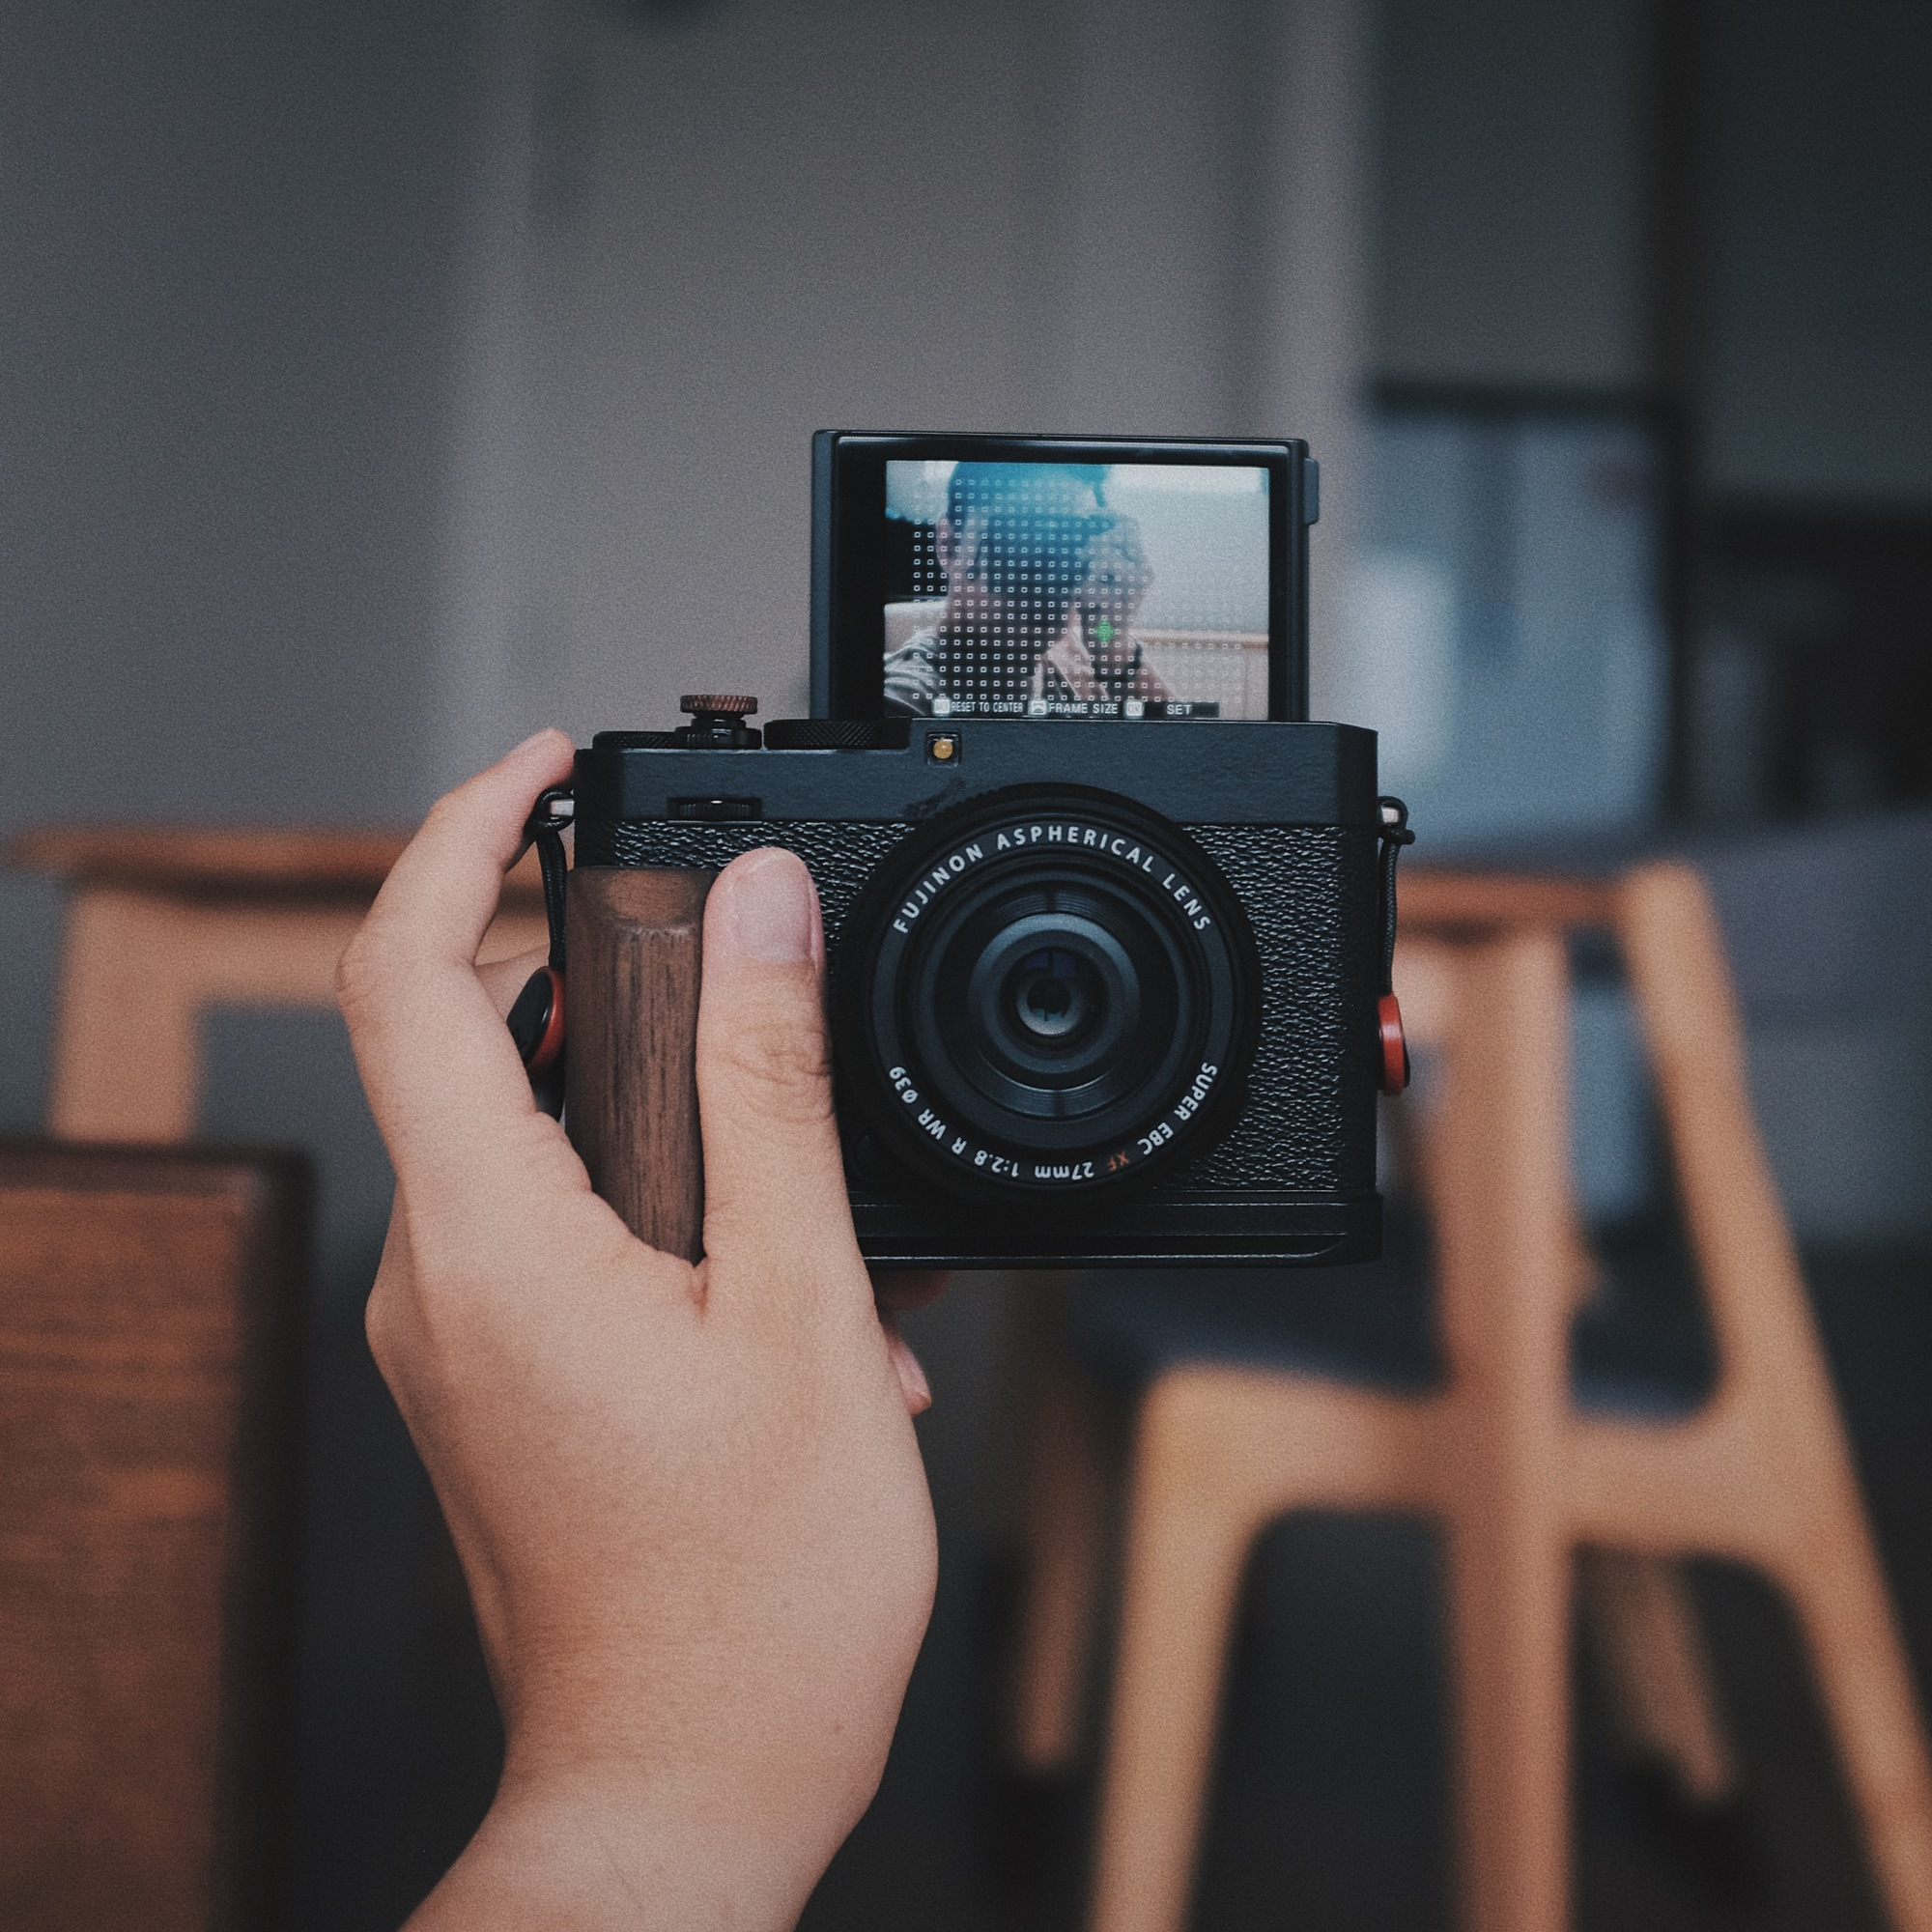
\includegraphics[width=\linewidth]{\envfinaldir/coverpic-prod.jpg}\par
            % \vskip 30pt
            \vfill

            \normalsize\rmfamily\scshape
            \copyright{} The Web Digest Project \hfill\large \envdatestr
        \end{center}
    \end{titlepage}
    % \restoregeometry
}
\newcommand{\simplehref}[1]{%
    \textcolor{blue!80!green}{\href{#1}{#1}}%
}
\renewcommand{\contentsname}{\center\Huge\sffamily\bfseries Contents\par\vskip 20pt}
\newcounter{ipartcounter}
\setcounter{ipartcounter}{0}
\newcommand{\ipart}[1]{
    % \vskip 20pt
    \clearpage
    \stepcounter{ipartcounter}
    \phantomsection
    \addcontentsline{toc}{chapter}{#1}
    % \begin{center}
    %     \Huge
    %     \sffamily\bfseries
    %     #1
    % \end{center}
    % \vskip 20pt plus 7pt
}
\newcounter{ichaptercounter}
\setcounter{ichaptercounter}{0}
\newcommand{\ichapter}[1]{
    % \vskip 20pt
    \clearpage
    \stepcounter{ichaptercounter}
    \phantomsection
    \addcontentsline{toc}{section}{\numberline{\arabic{ichaptercounter}}#1}
    \begin{center}
        \Huge
        \sffamily\bfseries
        #1
    \end{center}
    \vskip 20pt plus 7pt
}
\newcommand{\entrytitlefont}[1]{\subsection*{\raggedright\Large\sffamily\bfseries#1}}
\newcommand{\entryitemGeneric}[2]{
    % argv: title, url
    \parbox{\linewidth}{
        \entrytitlefont{#1}\par\vskip 5pt
        \footnotesize\ttfamily\mdseries
        \simplehref{#2}
    }\vskip 11pt plus 11pt minus 1pt
}
\newcommand{\entryitemGithub}[3]{
    % argv: title, url, desc
    \parbox{\linewidth}{
        \entrytitlefont{#1}\par\vskip 5pt
        \footnotesize\ttfamily\mdseries
        \simplehref{#2}\par\vskip 5pt
        \small\rmfamily\mdseries#3
    }\vskip 11pt plus 11pt minus 1pt
}
\newcommand{\entryitemAp}[3]{
    % argv: title, url, desc
    \parbox{\linewidth}{
        \entrytitlefont{#1}\par\vskip 5pt
        \footnotesize\ttfamily\mdseries
        \simplehref{#2}\par\vskip 5pt
        \small\rmfamily\mdseries#3
    }\vskip 11pt plus 11pt minus 1pt
}
\newcommand{\entryitemHackernews}[3]{
    % argv: title, hnurl, rawurl
    % \parbox{\linewidth}{
    %     \entrytitlefont{#1}\par\vskip 5pt
    %     \footnotesize\ttfamily\mdseries
    %     \simplehref{#3}\par
    %     \textcolor{black!50}{\href{#2}{#2}}
    % }\vskip 11pt plus 11pt minus 1pt
    \begin{minipage}{\linewidth}
            \entrytitlefont{#1}\par\vskip 5pt
            \footnotesize\ttfamily\mdseries
            \simplehref{#3}\par
            \textcolor{black!50}{\href{#2}{#2}}
    \end{minipage}\par\vskip 11pt plus 11pt minus 1pt
}







\begin{document}

\makeheader

\tableofcontents\clearpage




\ipart{Developers}
\ichapter{Hacker News}
\entryitemTwoLinks{The Burnout Machine}{https://news.ycombinator.com/item?id=43427002}{https://unionize.fyi}

\entryitemTwoLinks{OpenAI Audio Models}{https://news.ycombinator.com/item?id=43426022}{https://www.openai.fm/}

\entryitemTwoLinks{French scientist denied entry into the U.S., French government says}{https://news.ycombinator.com/item?id=43425841}{https://www.reuters.com/world/french-scientist-denied-entry-into-us-french-government-says-2025-03-20/}

\entryitemTwoLinks{Claude can now search the web}{https://news.ycombinator.com/item?id=43425655}{https://www.anthropic.com/news/web-search}

\entryitemTwoLinks{CVE-2024-54471: Leaking Passwords (and More!) on macOS}{https://news.ycombinator.com/item?id=43425605}{https://wts.dev/posts/password-leak/}

\entryitemTwoLinks{Canada considering charging for road access from USA to Alaska}{https://news.ycombinator.com/item?id=43425464}{https://washingtonstatestandard.com/2025/03/17/british-columbia-introduces-toll-measure-to-counter-tariffs/}

\entryitemTwoLinks{I fear for the unauthenticated web}{https://news.ycombinator.com/item?id=43424340}{https://sethmlarson.dev/i-fear-for-the-unauthenticated-web}

\entryitemTwoLinks{ACARS Drama}{https://news.ycombinator.com/item?id=43424065}{https://acarsdrama.com/}

\entryitemTwoLinks{Tesla falls after Commerce secretary recommends buying stock}{https://news.ycombinator.com/item?id=43423201}{https://www.axios.com/2025/03/20/tesla-musk-lutnick}

\entryitemTwoLinks{The Last Drops of Mexico City}{https://news.ycombinator.com/item?id=43423032}{https://mexicocitywater.longlead.com}

\entryitemTwoLinks{Oxygen discovered in most distant known galaxy}{https://news.ycombinator.com/item?id=43422909}{https://www.eso.org/public/news/eso2507/}

\entryitemTwoLinks{Tourist in US chained 'like Hannibal Lecter'}{https://news.ycombinator.com/item?id=43422551}{https://www.bbc.co.uk/news/articles/cly67j35y99o}

\entryitemTwoLinks{FOSS infrastructure is under attack by AI companies}{https://news.ycombinator.com/item?id=43422413}{https://thelibre.news/foss-infrastructure-is-under-attack-by-ai-companies/}

\entryitemTwoLinks{Tesla to recall more than 46,000 Cybertrucks due to exterior panel issue}{https://news.ycombinator.com/item?id=43422396}{https://www.cnn.com/2025/03/20/business/tesla-cybertruck-recall/index.html}

\entryitemTwoLinks{Ask HN: Are you afraid to travel to US to tech conferences?}{https://news.ycombinator.com/item?id=43422350}{https://news.ycombinator.com/item?id=43422350}

\entryitemTwoLinks{The Frontend Treadmill}{https://news.ycombinator.com/item?id=43422162}{https://polotek.net/posts/the-frontend-treadmill/}

\entryitemTwoLinks{Understanding Solar Energy}{https://news.ycombinator.com/item?id=43422033}{https://www.construction-physics.com/p/understanding-solar-energy}

\entryitemTwoLinks{Powers of 2 with all even digits}{https://news.ycombinator.com/item?id=43421934}{https://oeis.org/A068994}

\entryitemTwoLinks{Dutch Parliament: Time to ditch US tech for homegrown options}{https://news.ycombinator.com/item?id=43421902}{https://www.theregister.com/2025/03/19/dutch\_parliament\_us\_tech/}

\entryitemTwoLinks{EU sends Apple first DMA interoperability instructions for apps and devices}{https://news.ycombinator.com/item?id=43421740}{https://techcrunch.com/2025/03/19/eu-sends-apple-first-dma-interoperability-instructions-for-apps-and-connected-devices/}\ichapter{Phoronix}
\entryitemGeneric{\hskip 0pt{}The Most Interesting Linux 6.14 Features From NTSYNC To AMD Ryzen AI \& Rust Abstractions}{https://www.phoronix.com/news/Linux-6.14-Features-Reminder}

\entryitemGeneric{\hskip 0pt{}Mesa 25.0.2 Changes Range From Fixing Soft FP64 For Old AMD GPUs To RX 9070 Fixes}{https://www.phoronix.com/news/Mesa-25.0.2-Released}

\entryitemGeneric{\hskip 0pt{}Mesa RADV vs. AMDVLK Vulkan Driver Performance For The AMD Radeon RX 9070 Series}{https://www.phoronix.com/review/radeon-rx9070-radv-amdvlk}

\entryitemGeneric{\hskip 0pt{}Arm Bringing Up Support For Newer Mali GPUs With The Open-Source Panthor Driver}{https://www.phoronix.com/news/Arm-Mali-Newer-Hardware-Panthor}

\entryitemGeneric{\hskip 0pt{}Google Developing "Live Update Orchestrator" As New Means Of Live Linux Kernel Updates}{https://www.phoronix.com/news/Google-Live-Update-Orchestrator}

\entryitemGeneric{\hskip 0pt{}DAMON Self-Tuned Memory Tiering Shows Nice Improvement For Linux Servers}{https://www.phoronix.com/news/DAMON-Self-Tuned-Memory-Tiering}

\entryitemGeneric{\hskip 0pt{}Google Chrome Replacing FreeType With Rust-Written Skrifa For Font Handling}{https://www.phoronix.com/news/Google-Chrome-Going-Skrifa}

\entryitemGeneric{\hskip 0pt{}Miracle-WM 0.5 Released For Mir-Based Wayland Tiling Window Manager}{https://www.phoronix.com/news/Miracle-WM-0.5-Released}

\entryitemGeneric{\hskip 0pt{}SoftBank Acquiring ARM Server CPU Vendor Ampere Computing}{https://www.phoronix.com/news/SoftBank-Acquiring-Ampere}\ichapter{Dribbble}
\entryitemGeneric{\hskip 0pt{}Puzzle Fintech UI/UX design, User Interface experience}{https://dribbble.com/shots/25652036-Puzzle-Fintech-UI-UX-design-User-Interface-experience}

\entryitemGeneric{\hskip 0pt{}Novascan}{https://dribbble.com/shots/25790443-Novascan}

\entryitemGeneric{\hskip 0pt{}Sidebar Navigation for Core 2.0 – Dashboard Builder}{https://dribbble.com/shots/25790810-Sidebar-Navigation-for-Core-2-0-Dashboard-Builder}

\entryitemGeneric{\hskip 0pt{}Plain - Branding}{https://dribbble.com/shots/25790107-Plain-Branding}

\entryitemGeneric{\hskip 0pt{}Crypto Bridge}{https://dribbble.com/shots/25783744-Crypto-Bridge}

\entryitemGeneric{\hskip 0pt{}Eclipse - Logo Design}{https://dribbble.com/shots/25784396-Eclipse-Logo-Design}

\entryitemGeneric{\hskip 0pt{}Cargo Shipment App UI}{https://dribbble.com/shots/25784159-Cargo-Shipment-App-UI}

\entryitemGeneric{\hskip 0pt{}Burn Bright, Take Flight}{https://dribbble.com/shots/25778930-Burn-Bright-Take-Flight}

\entryitemGeneric{\hskip 0pt{}PieLabs Unused Logo Design}{https://dribbble.com/shots/25784372-PieLabs-Unused-Logo-Design}

\entryitemGeneric{\hskip 0pt{}The Planner app}{https://dribbble.com/shots/25769751-The-Planner-app}

\entryitemGeneric{\hskip 0pt{}Rose Logo Design [for sale]}{https://dribbble.com/shots/25775027-Rose-Logo-Design-for-sale}

\entryitemGeneric{\hskip 0pt{}Mammut Logo Redesign Concept}{https://dribbble.com/shots/25776663-Mammut-Logo-Redesign-Concept}

\entryitemGeneric{\hskip 0pt{}Cimet Logo Grid}{https://dribbble.com/shots/25710567-Cimet-Logo-Grid}

\entryitemGeneric{\hskip 0pt{}Bento grid \& dashboard for revops startup}{https://dribbble.com/shots/25765472-Bento-grid-dashboard-for-revops-startup}

\entryitemGeneric{\hskip 0pt{}Glide wallet}{https://dribbble.com/shots/25768771-Glide-wallet}

\entryitemGeneric{\hskip 0pt{}DL}{https://dribbble.com/shots/25775198-DL}

\entryitemGeneric{\hskip 0pt{}bigbeardamian: Badge Design}{https://dribbble.com/shots/25737398-bigbeardamian-Badge-Design}

\entryitemGeneric{\hskip 0pt{}Fitme}{https://dribbble.com/shots/25766813-Fitme}

\entryitemGeneric{\hskip 0pt{}Illustration}{https://dribbble.com/shots/25767159-Illustration}

\entryitemGeneric{\hskip 0pt{}Abstract S Logo Design // For Sale}{https://dribbble.com/shots/25764643-Abstract-S-Logo-Design-For-Sale}

\entryitemGeneric{\hskip 0pt{}Spin}{https://dribbble.com/shots/25765149-Spin}

\entryitemGeneric{\hskip 0pt{}Protec Recovery Logo Design}{https://dribbble.com/shots/25764203-Protec-Recovery-Logo-Design}

\entryitemGeneric{\hskip 0pt{}Fintech icons pack part 3 for download}{https://dribbble.com/shots/25728645-Fintech-icons-pack-part-3-for-download}

\entryitemGeneric{\hskip 0pt{}Capobara}{https://dribbble.com/shots/25764582-Capobara}


\ipart{Developers~~~~(zh-Hans)}
\ichapter{Solidot}
\entryitemGeneric{\hskip 0pt{}土耳其逮捕反对派领导人限制互联网}{https://www.solidot.org/story?sid=80836}

\entryitemGeneric{\hskip 0pt{}软银以 65 亿美元收购芯片设计公司 Ampere}{https://www.solidot.org/story?sid=80835}

\entryitemGeneric{\hskip 0pt{}鹦鹉如何模仿人类说话}{https://www.solidot.org/story?sid=80834}

\entryitemGeneric{\hskip 0pt{}PCI Express 7 即将完成,但 PCI Express 6 尚无普及}{https://www.solidot.org/story?sid=80833}

\entryitemGeneric{\hskip 0pt{}欧盟要求苹果开放生态系统否则将面临罚款}{https://www.solidot.org/story?sid=80832}

\entryitemGeneric{\hskip 0pt{}百度否认开盒信息来自该公司}{https://www.solidot.org/story?sid=80831}

\entryitemGeneric{\hskip 0pt{}Gemini 2.0 Flash 让任何人都能 PS}{https://www.solidot.org/story?sid=80830}

\entryitemGeneric{\hskip 0pt{}PC 玩家 92\% 的时间是在老游戏上}{https://www.solidot.org/story?sid=80829}

\entryitemGeneric{\hskip 0pt{}人类语言至少在 13.5 万年就存在}{https://www.solidot.org/story?sid=80828}

\entryitemGeneric{\hskip 0pt{}西班牙政治家对女性诉求的回应少于男性}{https://www.solidot.org/story?sid=80827}

\entryitemGeneric{\hskip 0pt{}SystemRescue 12.00 释出}{https://www.solidot.org/story?sid=80826}

\entryitemGeneric{\hskip 0pt{}Google 以 320 亿美元收购安全公司 Wiz}{https://www.solidot.org/story?sid=80825}

\entryitemGeneric{\hskip 0pt{}Eric Migicovsky 宣布推出两款运行 PebbleOS 的智能手表产品}{https://www.solidot.org/story?sid=80824}

\entryitemGeneric{\hskip 0pt{}密码复用攻击泛滥成灾}{https://www.solidot.org/story?sid=80823}

\entryitemGeneric{\hskip 0pt{}波音 Starliner 宇航员返回地面}{https://www.solidot.org/story?sid=80822}

\entryitemGeneric{\hskip 0pt{}欧洲科技公司呼吁欧盟推动购买欧洲科技产品}{https://www.solidot.org/story?sid=80821}

\entryitemGeneric{\hskip 0pt{}人类的脑力已经越过峰值?}{https://www.solidot.org/story?sid=80820}

\entryitemGeneric{\hskip 0pt{}周五是否应该成为新的周六?}{https://www.solidot.org/story?sid=80819}

\entryitemGeneric{\hskip 0pt{}哈佛对年收入 20 万美元以内家庭免除学费}{https://www.solidot.org/story?sid=80818}

\entryitemGeneric{\hskip 0pt{}百度副总裁的未成年女儿被指参与开盒}{https://www.solidot.org/story?sid=80817}\ichapter{V2EX}
\entryitemGeneric{\hskip 0pt{}[iPhone] 耳机里的 siri 播报声音如何降低}{https://www.v2ex.com/t/1120007}

\entryitemGeneric{\hskip 0pt{}[Windows] windows 资源管理器 如何添加预览得文件格式呢}{https://www.v2ex.com/t/1120006}

\entryitemGeneric{\hskip 0pt{}[创业组队] 游戏+聊天室出海}{https://www.v2ex.com/t/1120005}

\entryitemGeneric{\hskip 0pt{}[Android] 安卓上有些国际毒瘾利用 FCM 不断拉起 App 后台活动,好像没办法压?}{https://www.v2ex.com/t/1120004}

\entryitemGeneric{\hskip 0pt{}[程序员] 为什么 Python 、Node.js 就不能学习一下 C\#这种优雅的依赖管理方式?}{https://www.v2ex.com/t/1120003}

\entryitemGeneric{\hskip 0pt{}[职场话题] 坐标望京说下大龄 RD 同事前同事的找工作情况吧-250321}{https://www.v2ex.com/t/1120002}

\entryitemGeneric{\hskip 0pt{}[微信] 微信小程序开发的小活 外包}{https://www.v2ex.com/t/1120000}

\entryitemGeneric{\hskip 0pt{}[程序员] 如何入门 AI 辅助编程}{https://www.v2ex.com/t/1119999}

\entryitemGeneric{\hskip 0pt{}[酷工作] [远程] Android 开发工程师/iOS 开发工程师/ QA 测试工程师/ WEB 前端工程师 [GiggleAcademy]}{https://www.v2ex.com/t/1119998}

\entryitemGeneric{\hskip 0pt{}[问与答] 国行有没有可以刷欧版系统后所有功能正常的 android 手机?}{https://www.v2ex.com/t/1119997}

\entryitemGeneric{\hskip 0pt{}[职场话题] 帮老婆在其公司打抱不平. 分享一波 (重置分段版)}{https://www.v2ex.com/t/1119996}

\entryitemGeneric{\hskip 0pt{}[天黑以后] 20250320 午夜俱乐部}{https://www.v2ex.com/t/1119995}

\entryitemGeneric{\hskip 0pt{}[优惠信息] 慢收 苹果妙控键盘和妙控板}{https://www.v2ex.com/t/1119994}

\entryitemGeneric{\hskip 0pt{}[职场话题] 巴掌大的公司的定薪流程模板}{https://www.v2ex.com/t/1119993}

\entryitemGeneric{\hskip 0pt{}[职场话题] 有哪些在职的比较好办理而失业状态不太好办理的证件/手续呢?}{https://www.v2ex.com/t/1119992}

\entryitemGeneric{\hskip 0pt{}[iDev] [请教] iOS 开发,如何查询和更新内支付价格到最新汇率}{https://www.v2ex.com/t/1119991}

\entryitemGeneric{\hskip 0pt{}[职场话题] 帮老婆在其公司打抱不平. 分享一波}{https://www.v2ex.com/t/1119990}

\entryitemGeneric{\hskip 0pt{}[职场话题] 武汉金山云 offer 如何}{https://www.v2ex.com/t/1119989}

\entryitemGeneric{\hskip 0pt{}[问与答] win 系统上有什么可以编写 md 格式程序吗?}{https://www.v2ex.com/t/1119988}

\entryitemGeneric{\hskip 0pt{}[Apple] 新买的 MacBook Air 不小心摔了怎么办}{https://www.v2ex.com/t/1119987}

\entryitemGeneric{\hskip 0pt{}[宽带症候群] 装修网络布局}{https://www.v2ex.com/t/1119986}

\entryitemGeneric{\hskip 0pt{}[宽带症候群] L2TP 已经被搞?}{https://www.v2ex.com/t/1119985}

\entryitemGeneric{\hskip 0pt{}[问与答] 焦虑症萌新关于 CloudFlare 删除域名 和 ZeroTrust 的问题,求助!}{https://www.v2ex.com/t/1119984}

\entryitemGeneric{\hskip 0pt{}[程序员] coding.net 免费版要停了,大家会换哪个平台呢?}{https://www.v2ex.com/t/1119983}

\entryitemGeneric{\hskip 0pt{}[随想] 今天总算是把 V2 的摸鱼进度条打满了}{https://www.v2ex.com/t/1119982}

\entryitemGeneric{\hskip 0pt{}[分享创造] 做了一个设计编辑器,主打批量生成,不用再为 canva 付钱了}{https://www.v2ex.com/t/1119981}

\entryitemGeneric{\hskip 0pt{}[问与答] e-CNY 数字货币已经烂尾了吗}{https://www.v2ex.com/t/1119980}

\entryitemGeneric{\hskip 0pt{}[Apple] 新 iPhone 无法激活 FaceTime 和 iMessage,中国电信}{https://www.v2ex.com/t/1119979}

\entryitemGeneric{\hskip 0pt{}[分享创造] Fetcher MCP: MCP 服务器,用于使用 Playwright 无头浏览器获取网页内容。}{https://www.v2ex.com/t/1119976}

\entryitemGeneric{\hskip 0pt{}[分享发现] kodi 只能看到 windows 共享文件中部分文件问题}{https://www.v2ex.com/t/1119974}

\entryitemGeneric{\hskip 0pt{}[程序员] 大家怎么看用 saas 模板来快速搭建网站?}{https://www.v2ex.com/t/1119973}

\entryitemGeneric{\hskip 0pt{}[分享发现] 分享一下线上配镜体验}{https://www.v2ex.com/t/1119972}

\entryitemGeneric{\hskip 0pt{}[全球工单系统] 瀚思彼岸 不在线了吗?}{https://www.v2ex.com/t/1119971}

\entryitemGeneric{\hskip 0pt{}[程序员] 请问各位有什么更推荐的影片文件的 m3u8 和 key 分离的方案吗}{https://www.v2ex.com/t/1119970}

\entryitemGeneric{\hskip 0pt{}[问与答] twitter 账号被封禁了,怎么申诉也不给解封,充会员的话能吗}{https://www.v2ex.com/t/1119969}

\entryitemGeneric{\hskip 0pt{}[问与答] 求批量安装电脑系统教程}{https://www.v2ex.com/t/1119968}

\entryitemGeneric{\hskip 0pt{}[路由器] 华为的家用路由器 AX2Pro,居然连自定义掩码都不支持}{https://www.v2ex.com/t/1119967}

\entryitemGeneric{\hskip 0pt{}[问与答] one drive 和 dropbox,我该选哪个?}{https://www.v2ex.com/t/1119966}

\entryitemGeneric{\hskip 0pt{}[程序员] 想知道大家工作中力扣 Hot100 里的哪个算法在业务逻辑里会用的比较多?为什么?}{https://www.v2ex.com/t/1119965}

\entryitemGeneric{\hskip 0pt{}[程序员] twillot,一个挺好用的 twitter 内容整理的插件}{https://www.v2ex.com/t/1119964}

\entryitemGeneric{\hskip 0pt{}[程序员] 现在有人用 TDD 测试驱动来配合 AI 开发吗}{https://www.v2ex.com/t/1119963}

\entryitemGeneric{\hskip 0pt{}[程序员] 探索 MCP-我的学习与实践笔记}{https://www.v2ex.com/t/1119962}

\entryitemGeneric{\hskip 0pt{}[Docker] 求助, docker inspect 命令查出的 Pid 不存在}{https://www.v2ex.com/t/1119961}

\entryitemGeneric{\hskip 0pt{}[NAS] 飞牛 OS N150 虚拟化核显不工作}{https://www.v2ex.com/t/1119960}

\entryitemGeneric{\hskip 0pt{}[程序员] windsurf 买了 pro ,每天也有调用上限吗}{https://www.v2ex.com/t/1119959}

\entryitemGeneric{\hskip 0pt{}[职场话题] 6 年产品被裁两周拿到一家小公司 offer 要不要去?}{https://www.v2ex.com/t/1119957}

\entryitemGeneric{\hskip 0pt{}[职场话题] 大哥们帮忙选一下 offer}{https://www.v2ex.com/t/1119956}

\entryitemGeneric{\hskip 0pt{}[Android] Android 应用使用情况 事件不完整了 我就说吧}{https://www.v2ex.com/t/1119955}

\entryitemGeneric{\hskip 0pt{}[Firefox] firefox 136 不支持 WebCodecs API 中调用 265 相关的解码器吗?}{https://www.v2ex.com/t/1119954}

\entryitemGeneric{\hskip 0pt{}[奇思妙想] 想法被华为重新实现了一下,人生圆满了}{https://www.v2ex.com/t/1119953}


\ipart{Generic News}
\ichapter{AP News}
\entryitemWithDescription{\hskip 0pt{}Mariah Carey didn't steal `All I Want For Christmas Is You' from other writers, a judge says}{https://apnews.com/article/11bd38db45f8e248711ab85c0803b026}{}

\entryitemWithDescription{\hskip 0pt{}In latest blow to Tesla, regulators recall nearly all Cybertrucks}{https://apnews.com/article/8c517e21aa1119d74b9db39f6aca01b7}{}

\entryitemWithDescription{\hskip 0pt{}Hawaii's Kilauea volcano resumes dazzling show with lava fountains hundreds of feet high}{https://apnews.com/article/bc7c2f45805b663ce6e448ad4b582517}{}

\entryitemWithDescription{\hskip 0pt{}An Italian beach town in Tuscany is invaded by midges. Residents seek emergency declaration to cope}{https://apnews.com/article/1743293cff18033ac0404083c1873f6d}{}

\entryitemWithDescription{\hskip 0pt{}New York's top court blocks NYC from letting noncitizens vote}{https://apnews.com/article/30c65e13fc81136650606a37e17ed88d}{}

\entryitemWithDescription{\hskip 0pt{}Amtrak CEO abruptly resigns from the nation's passenger railroad}{https://apnews.com/article/a57e28dfe402dabe3fad68294c1e6818}{}

\entryitemWithDescription{\hskip 0pt{}Delta plane that flipped over in Toronto last month showed high rate of descent, initial report says}{https://apnews.com/article/39f9a9f78533296bb72a95161a37056f}{}

\entryitemWithDescription{\hskip 0pt{}Government cannot deport Georgetown scholar until court rules, judge orders}{https://apnews.com/article/21fc205cebbbbba2ed260050df04702a}{}

\entryitemWithDescription{\hskip 0pt{}NBA champ Celtics sold for record \$6.1 billion to group led by private equity mogul Bill Chisholm}{https://apnews.com/article/c8d050f615af7563c71ffe1f7601825d}{}

\entryitemWithDescription{\hskip 0pt{}Venus passes between the Earth and sun this weekend — but don't try to look for it}{https://apnews.com/article/0b31d37604fec1721f8f60505f50b986}{}

\entryitemWithDescription{\hskip 0pt{}XRP jumps 8\% after Ripple's CEO says SEC has dropped its case against the crypto currency}{https://apnews.com/article/02bb5d70c23864db2421d4b70cf4cea0}{}

\entryitemWithDescription{\hskip 0pt{}Hawaii's Kilauea volcano resumes on-and-off again eruption that has dazzled park visitors}{https://apnews.com/article/43504dd7223e1e9d6714fbc2cbfb392c}{}

\entryitemWithDescription{\hskip 0pt{}A former studio engineer is charged with stealing unreleased Eminem music and selling it online}{https://apnews.com/article/6b707ffbada116baf9c0042d12675244}{}






\clearpage
\leavevmode\vfill
\footnotesize

Copyright \copyright{} 2023-2025 Neruthes and other contributors.

This document is published with CC BY-NC-ND 4.0 license.

The entries listed in this newsletter may be copyrighted by their respective creators.

This newsletter is generated by the Web Digest project.

The newsletters are also delivered via Telegram channel \CJKunderline{\href{https://t.me/webdigestchannel}{https://t.me/webdigestchannel}}.\\
RSS feed is available at \CJKunderline{\href{https://webdigest.pages.dev/rss.xml}{https://webdigest.pages.dev/rss.xml}}.

This newsletter is available in PDF at
\CJKunderline{\href{https://webdigest.pages.dev/}{https://webdigest.pages.dev/}}.

The source code being used to generate this newsletter is available at\\
\CJKunderline{\href{https://github.com/neruthes/webdigest}{https://github.com/neruthes/webdigest}}.

This newsletter is also available in
\CJKunderline{\href{http://webdigest.pages.dev/readhtml/\envyear/WebDigest-20250321.html}{HTML}} and
\CJKunderline{\href{https://github.com/neruthes/webdigest/blob/master/markdown/\envyear/WebDigest-20250321.md}{Markdown}}.


\coverpic{https://unsplash.com/photos/a-blurry-image-of-a-purple-object-in-the-dark-qktO9NjK\_Ak}{Zoha Gohar}


\end{document}
